\chapter{动力系统}
\label{cha:Motor}

\section{双极型步进电机}

\begin{figure}[htbp]
    \centering
    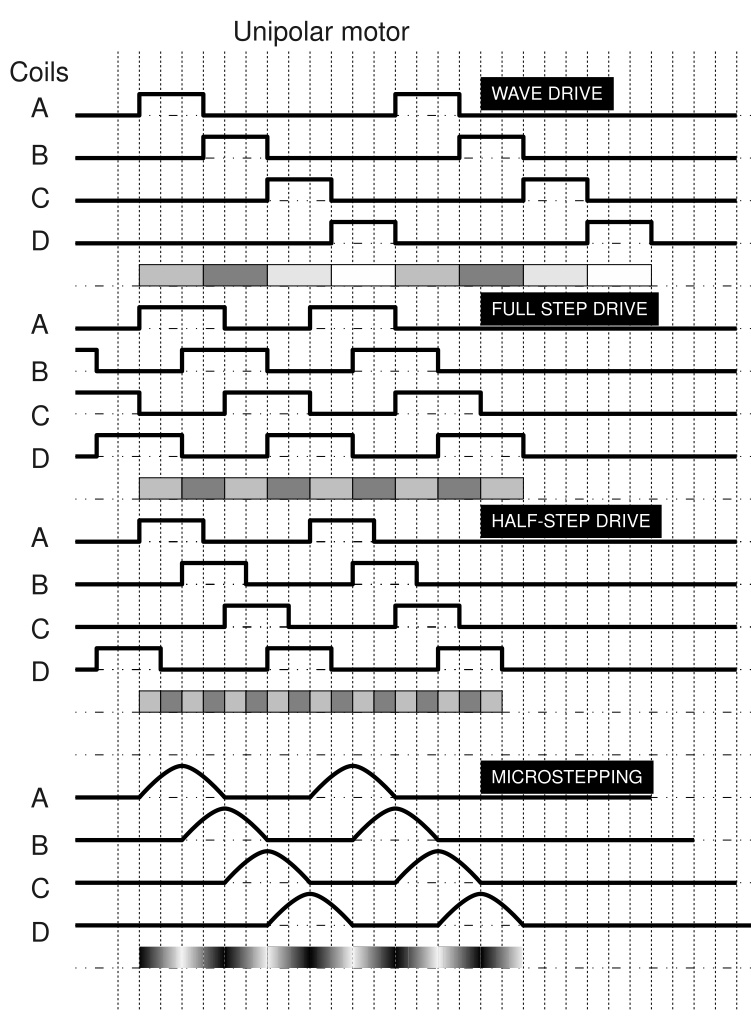
\includegraphics[width=\columnwidth]{Drive.png}
    \caption{Phase current waveforms}
    \label{fig:Phase-current}
\end{figure}

双极步进电机(Bipolar motors\footnote{\url{https://en.wikipedia.org/wiki/Stepper_motor}})每相只有一个绕组。为了使磁极反向,需要使绕组中的电流反向,因此驱动电路必须更复杂,通常采用H桥配置(但是有几种现成的驱动器芯片可以使之成为一个简单的事情)。每相有两个引线,没有公用的。

两线圈双极步进步进电机的典型驱动模式为:A + B + A- B-。即以正电流驱动线圈A,然后从线圈A中去除电流。然后以正电流驱动线圈B,然后从线圈B中去除电流。然后用负电流驱动线圈A(通过切换导线,例如用H桥翻转极性),然后从线圈A去除电流。然后用负电流驱动线圈B(与线圈A的翻转极性相同);循环完成并重新开始。

由于更好地利用了绕组,因此它们比同等重量的单极步进电机更强大。这是由于绕组占用的物理空间。单极电机在相同的空间中具有两倍的导线数量,但在任何时间点仅使用一半的导线,因此效率为50\%(或大约70\%的可用扭矩输出)。尽管双极步进电机的驱动更加复杂,但丰富的驱动芯片简化了实际使用时的复杂度。

\section{步进电机驱动}

斩波驱动电路(Chopper drive circuits)称为受控电流驱动器,因为它们在每个绕组中产生受控电流,而不是施加恒定电压。斩波器驱动电路最常用于双绕组双极步进电机,两个绕组被独立驱动以提供特定的步进电机转矩CW或CCW。在每个绕组上,将“电源”电压作为方波电压施加到绕组上。例如8 kHz。绕组电感使电流平滑,该电流达到根据方波占空比的水平。相对于绕组回路,双极性电源(+和-)电压通常提供给控制器。

\section{步进电机驱动DRV8825}

DRV8825用于双极步进电机控制。微步步进电机驱动器提供更高的精度以及步进电机平稳的旋转。

\begin{figure}[htbp]
    \centering
    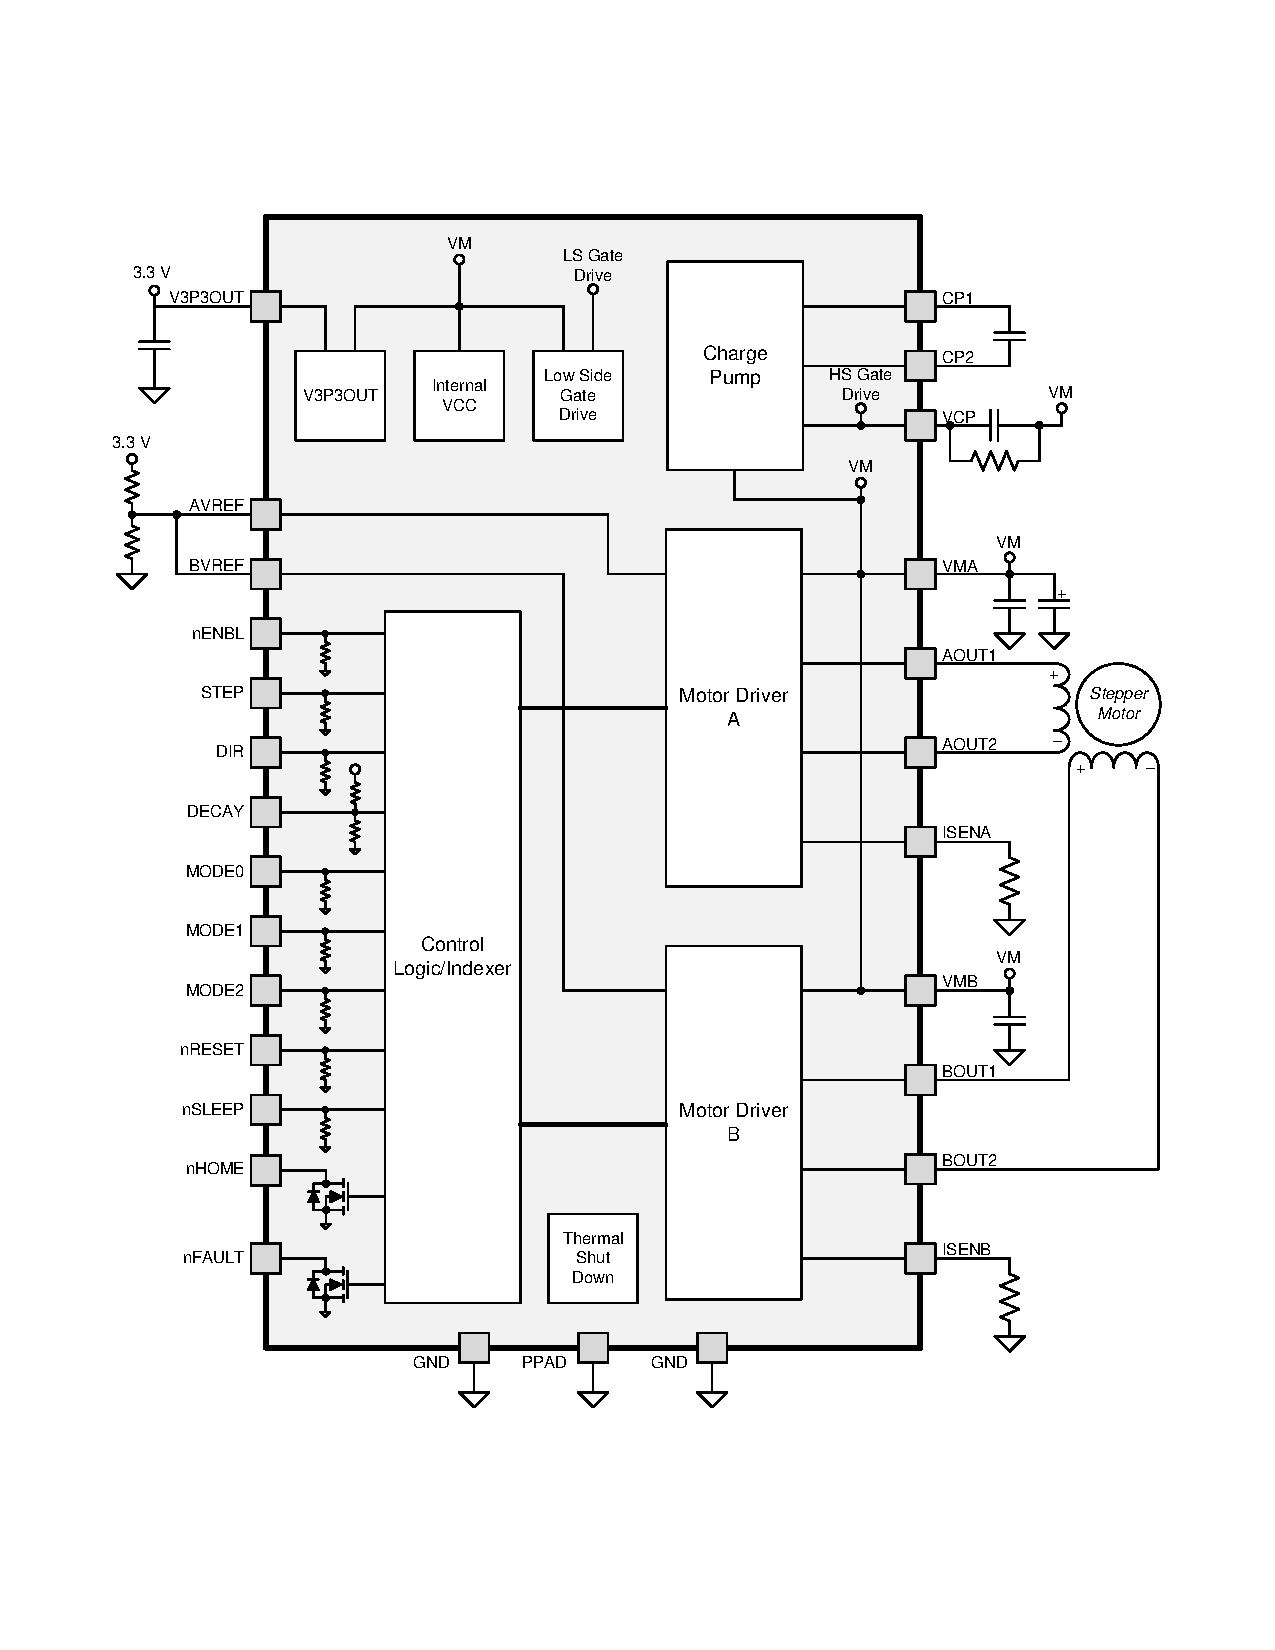
\includegraphics[width=\columnwidth]{DRV8825-Function-Block.pdf}
    \caption{DRV8825功能框图}
    \label{fig:DRV8825-Function-Block}
\end{figure}

配置DRV8825的第一步需要所需的转速和微步级别。

\begin{figure}[htbp]
    \centering
    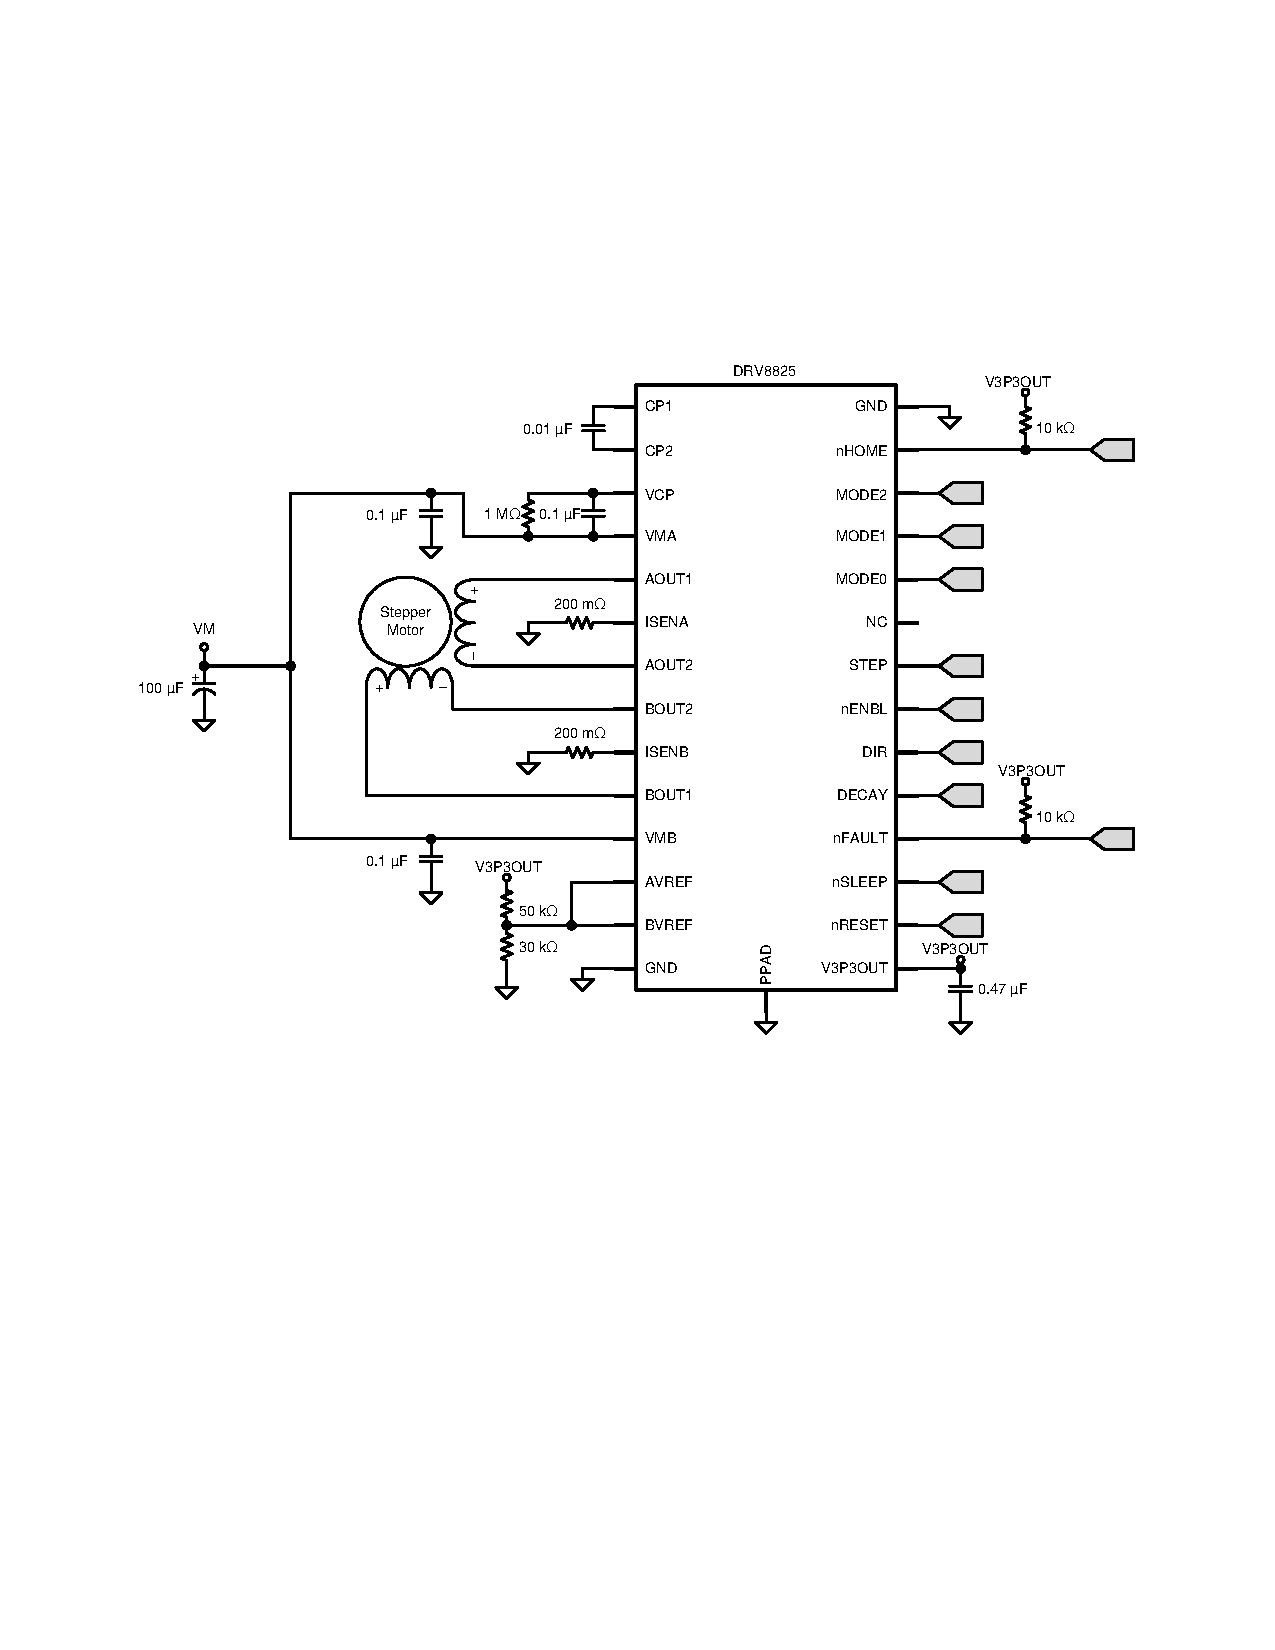
\includegraphics[width=\columnwidth]{DRV8825-Typical-Application.pdf}
    \caption{DRV8825典型应用}
    \label{fig:DRV8825-Typical-Application}
\end{figure}


\begin{figure}[htbp]
    \centering
    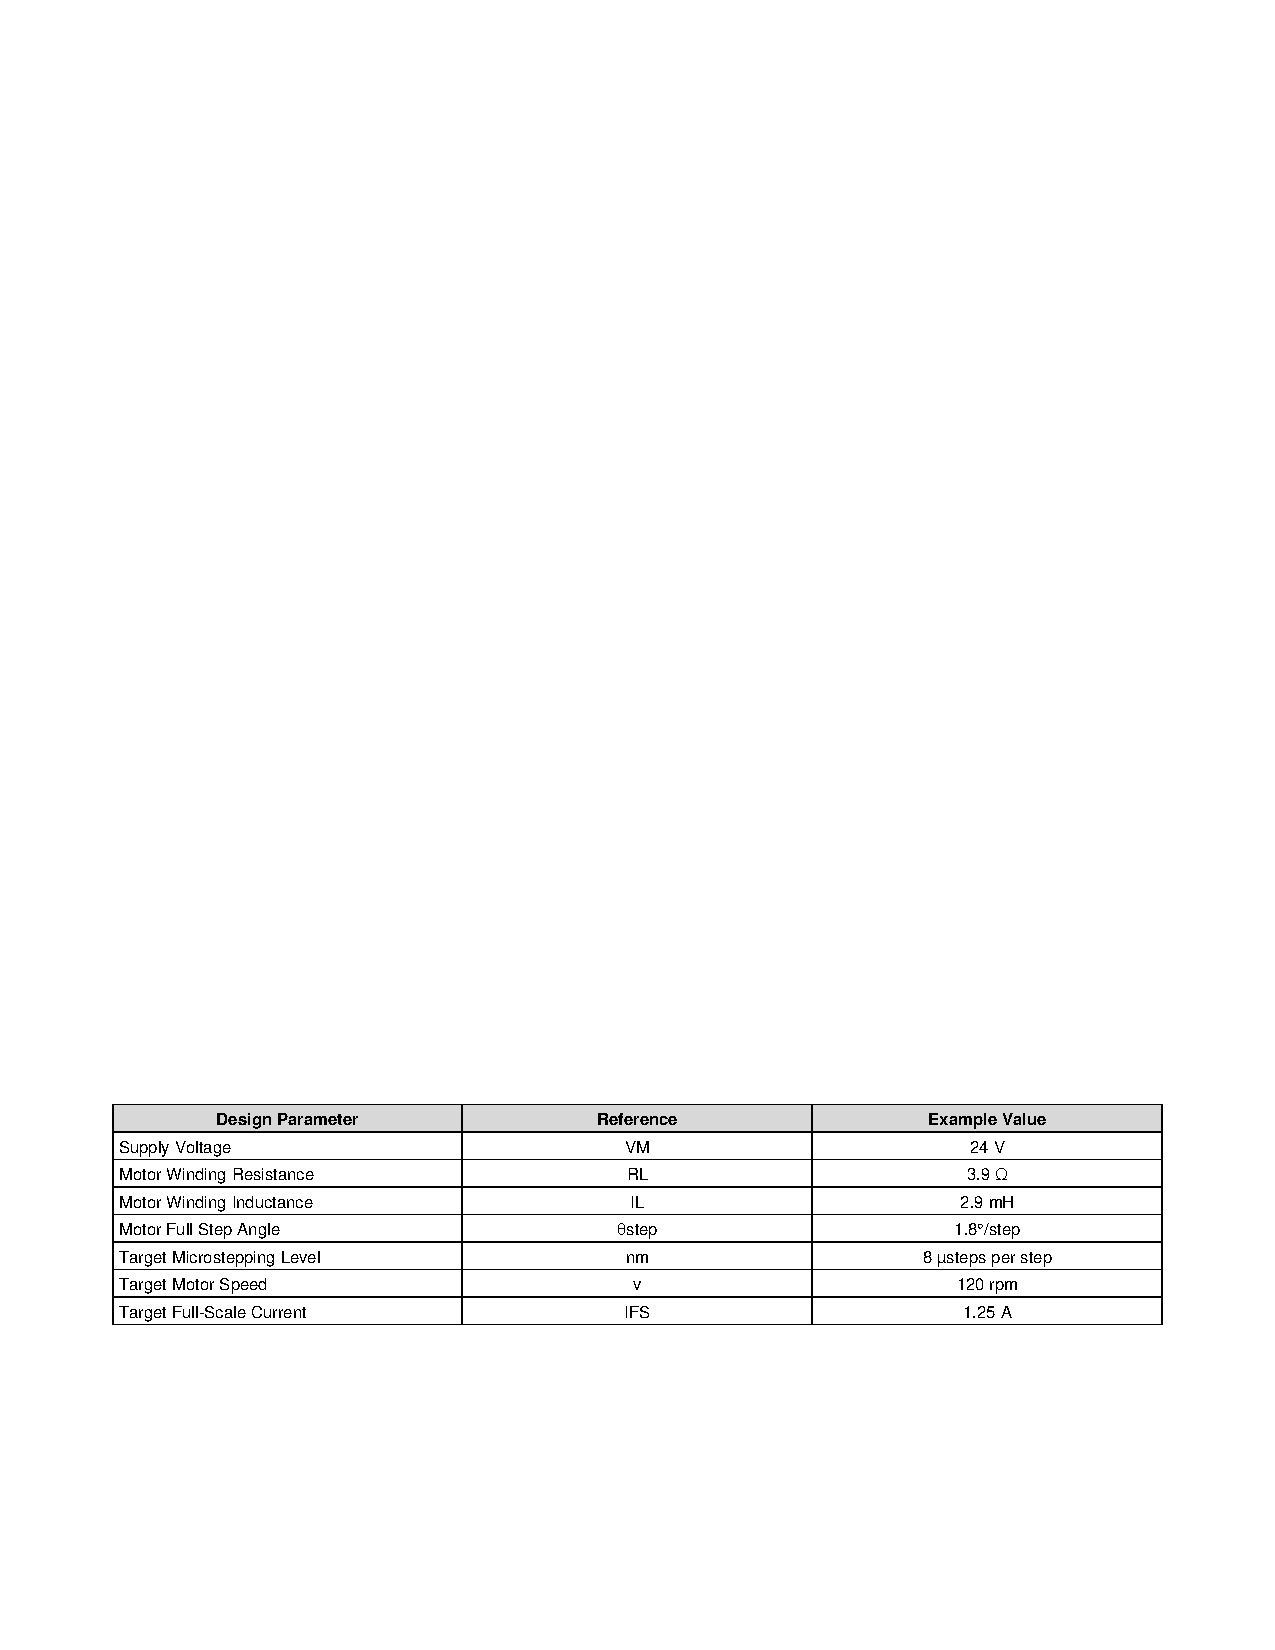
\includegraphics[width=\columnwidth]{DRV8825-Design-Requirements.pdf}
    \caption{DRV8825设计要求}
    \label{fig:DRV8825-Design-Requirements}
\end{figure}

如果需要恒定转速,则将频率为$f_step$的方波施加到STEP引脚。

如果步进电机的目标速度过高,步进电机可能不会旋转。 确保步进电机可以支持目标速度或通过加速以使步进电机达到最高速度。

对于所需的步进电机速度(v),微步级别($n_m$)和步进电机全步距角($\theta_{\text {step }}$,一整步对应的角度),

\begin{equation}
    \begin{aligned}
    &f_{\text {step }(\mu \text { steps } / \text { second })=} \frac{v\left(\frac{\text { rotations }}{\text { minute }}\right) \times 360\left(\frac{\circ}{\text { rotation }}\right) \times n_{\mathrm{m}}\left(\frac{\mu \text { steps }}{\text { step }}\right)}{60\left(\frac{\text { seconds }}{\text { minute }}\right) \times \theta_{\text {step }}\left(\frac{^{\circ}}{\text { step }}\right)}\\
    &f_{\text {step }(\mu \text { steps } / \text { second })=} \frac{120\left(\frac{\text { rotations }}{\text { minute }}\right) \times 360\left(\frac{^{\circ}}{\text { rotation }}\right) \times 8\left(\frac{\mu \text { steps }}{\text { step }}\right)}{60\left(\frac{\text { seconds }}{\text { minute }}\right) \times 1.8\left(\frac{\circ}{\text { step }}\right)}
    \end{aligned}
\end{equation}

DRV8825微步步进级别由MODE引脚设置。

较高的微步步进级别将意味着步进电机运动更平稳且噪声较小,但会增加开关损耗,并且需要较高的$f_step$才能达到相同的步进电机速度。

在步进电机中,设定的满量程电流($I_{FS}$ full-scale current)是通过任一绕组驱动的最大电流。 该数量取决于xVREF模拟电压和检测电阻值($R_{\text {SENSE}}$)。 

在步进期间,IFS定义为最大电流步进斩波阈值($I_{\text {TRIP}}$ current chopping threshold)。 DRV8825的增益设置为5V。

\begin{equation}
    \operatorname{I_{FS}}(A)=\frac{x \operatorname{VREF}(V)}{A_{v} \times R_{S E N S E}(\Omega)}=\frac{x \operatorname{VREF}(V)}{5 \times R_{S E N S E}(\Omega)}
\end{equation}

参考设计和要求如图~\ref{fig:DRV8825-Typical-Application}和图~\ref{fig:DRV8825-Design-Requirements}

典型模块设计和布局如图~\ref{fig:DRV8825-stepper-motor-driver-carrier-schematic-diagram}和图~\ref{fig:DRV8825-Layout-Example}

\begin{figure}[htbp]
    \centering
    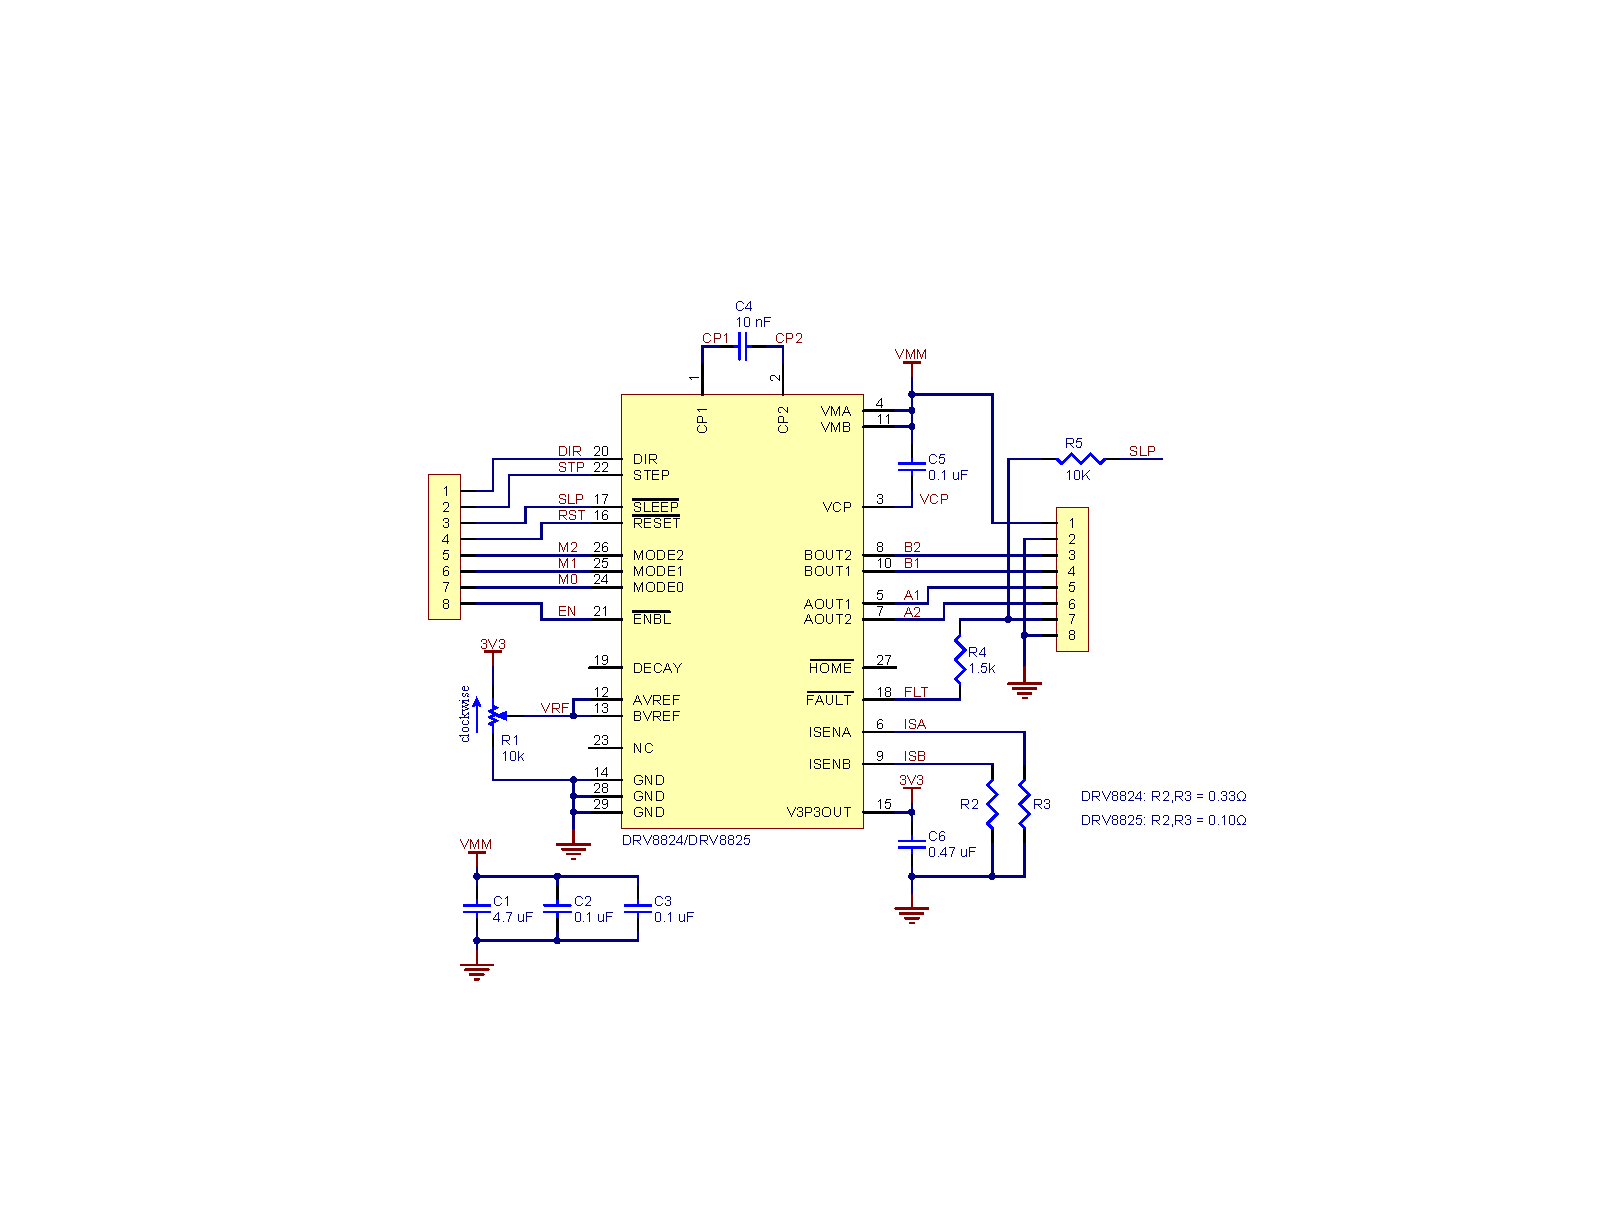
\includegraphics[width=\columnwidth]{drv8824-drv8825-stepper-motor-driver-carrier-schematic-diagram.pdf}
    \caption{DRV8825模块设计 DRV8824/DRV8825 Stepper Motor Driver Carrier}
    \label{fig:DRV8825-stepper-motor-driver-carrier-schematic-diagram}
\end{figure}

\begin{figure}[htbp]
    \centering
    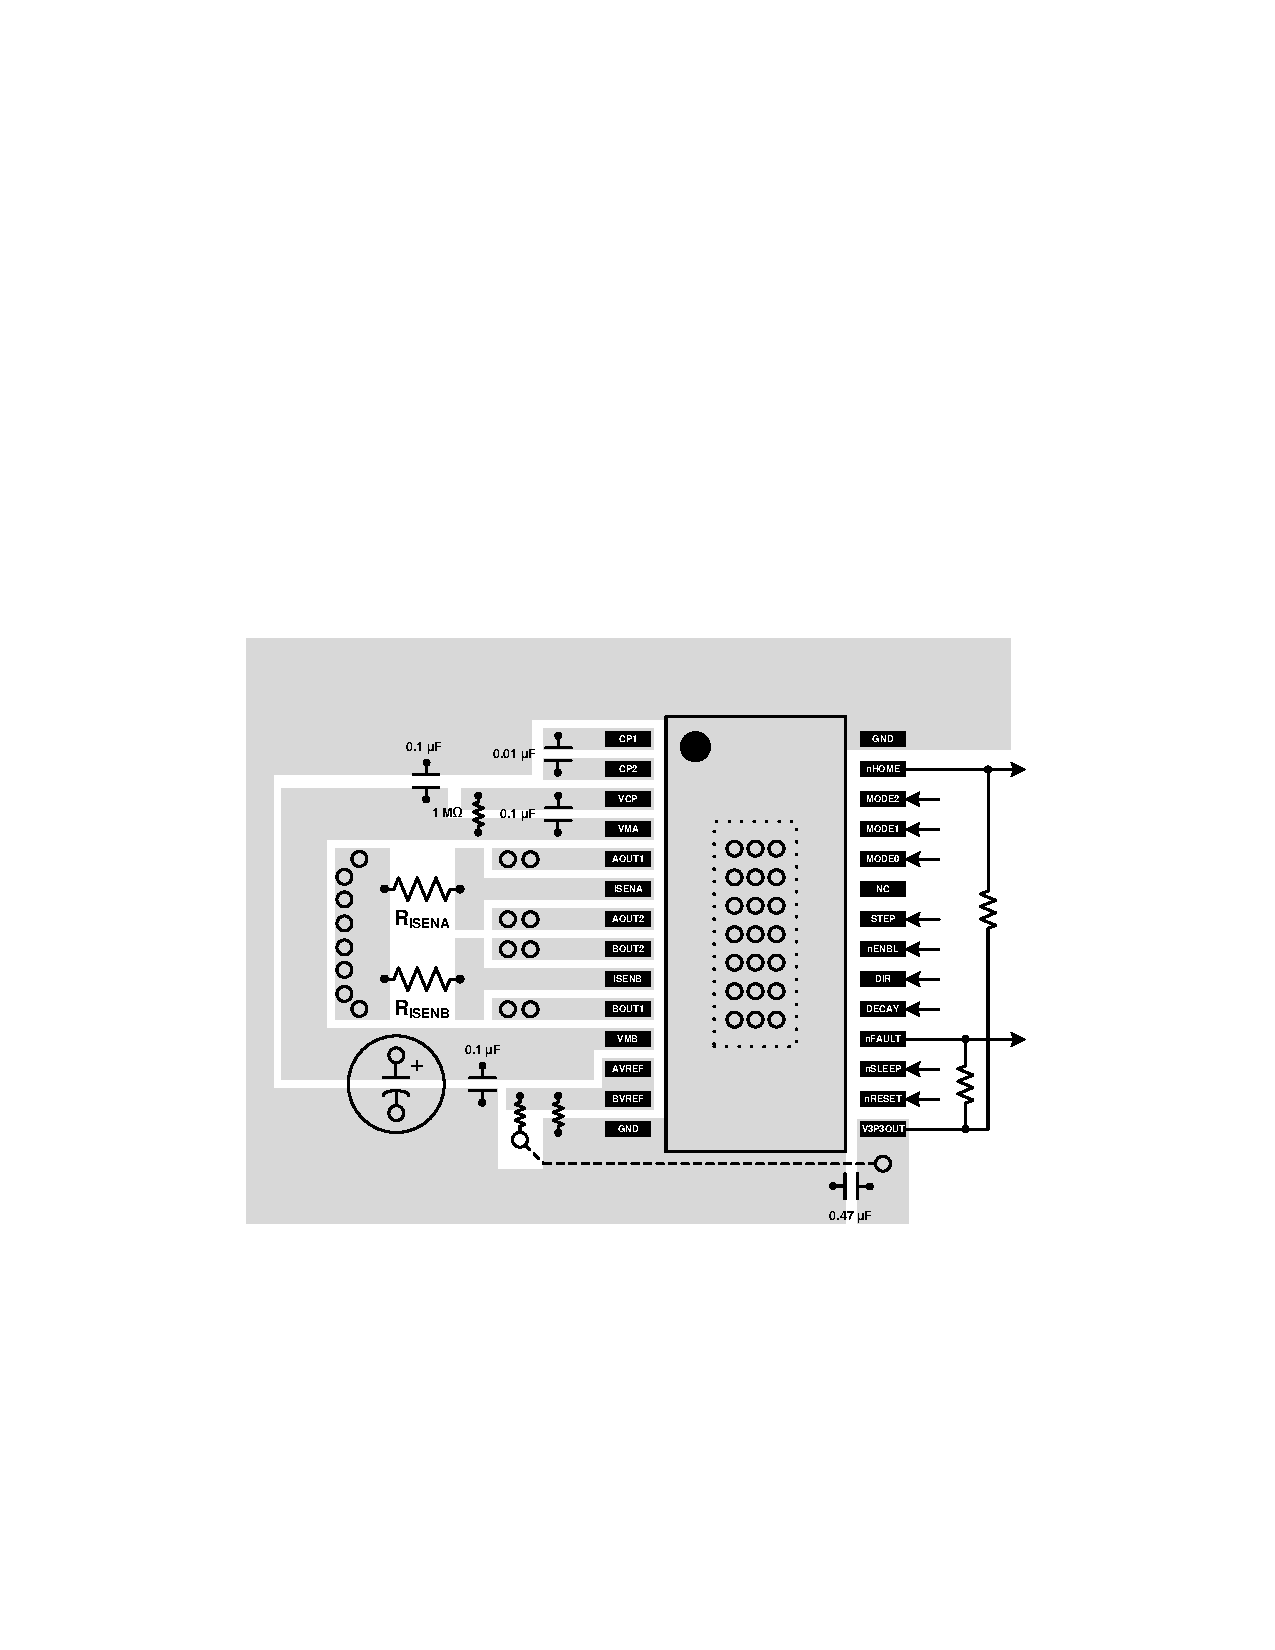
\includegraphics[width=\columnwidth]{DRV8825-Layout-Example.pdf}
    \caption{DRV8825布局参考}
    \label{fig:DRV8825-Layout-Example}
\end{figure}


\section{减速步进电机}

CHS-GM1024-10BY 2相4线直径15BY全金属齿轮减速步进电机 参数如图~\ref{fig:CHS-GM1024-10BY-Specific}所示。

\begin{figure}[htbp]
    \centering
    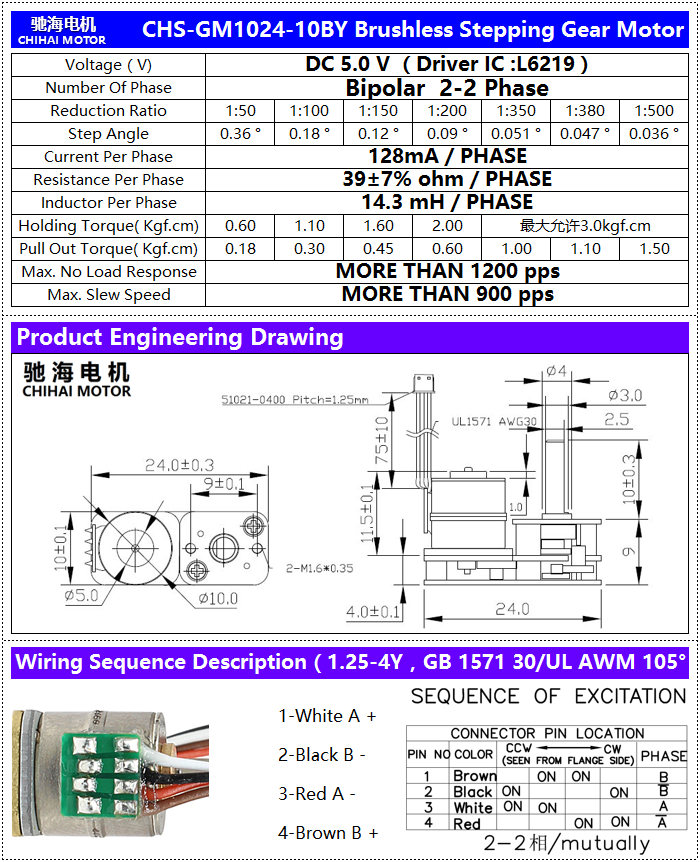
\includegraphics[width=\columnwidth]{CHS-GM1024-10BY-Specific.jpg}
    \caption{CHS-GM1024-10BY参数}
    \label{fig:CHS-GM1024-10BY-Specific}
\end{figure}

\begin{table}[htbp]
    \centering
    \begin{tabular}{ll}
    \hline
    Model                  & CHS-GM1024-10BY   \\ \hline
    Working voltage        & DC 5V             \\ \hline
    Phase                  & 2 phase 4 wire    \\ \hline
    Reduction ratio        & 1:100             \\ \hline
    Step angle             & 0.18°             \\ \hline
    Phase current          & 128mA/phase       \\ \hline
    Phase resistance       & 39±7\%ohm/phase   \\ \hline
    Phase inductance       & 14.3mH/phase      \\ \hline
    Holding torque         & 1.10kgf.cm        \\ \hline
    Pull out torque        & 0.30kgf.cm        \\ \hline
    Max starting frequency & More than 1200pps \\ \hline
    Response frequency     & More than 900pps  \\ \hline
    \end{tabular}
    \caption{CHIHAI MOTOR DC 5V Brushless Motor 2 Phase 4 Wire Stepper Motor Specification}
    \label{tab:CHS-GM1024-10BY-Specific}
\end{table}

\section{电机连接器}

采用的电机原装为Molex 51021-0400 连接器 1.25mm Pitch, PicoBlade 1.25 DIP TYPE SMT TYPE \url{https://www.chinese.molex.com/molex/products/part-detail/crimp_housings/0510210400},为了方便未来批量制作,我们使用对应的插座,如图~\ref{fig:51021-APPLICATION-SPECIFICATION}所示。

\begin{figure}[htbp]
    \centering
    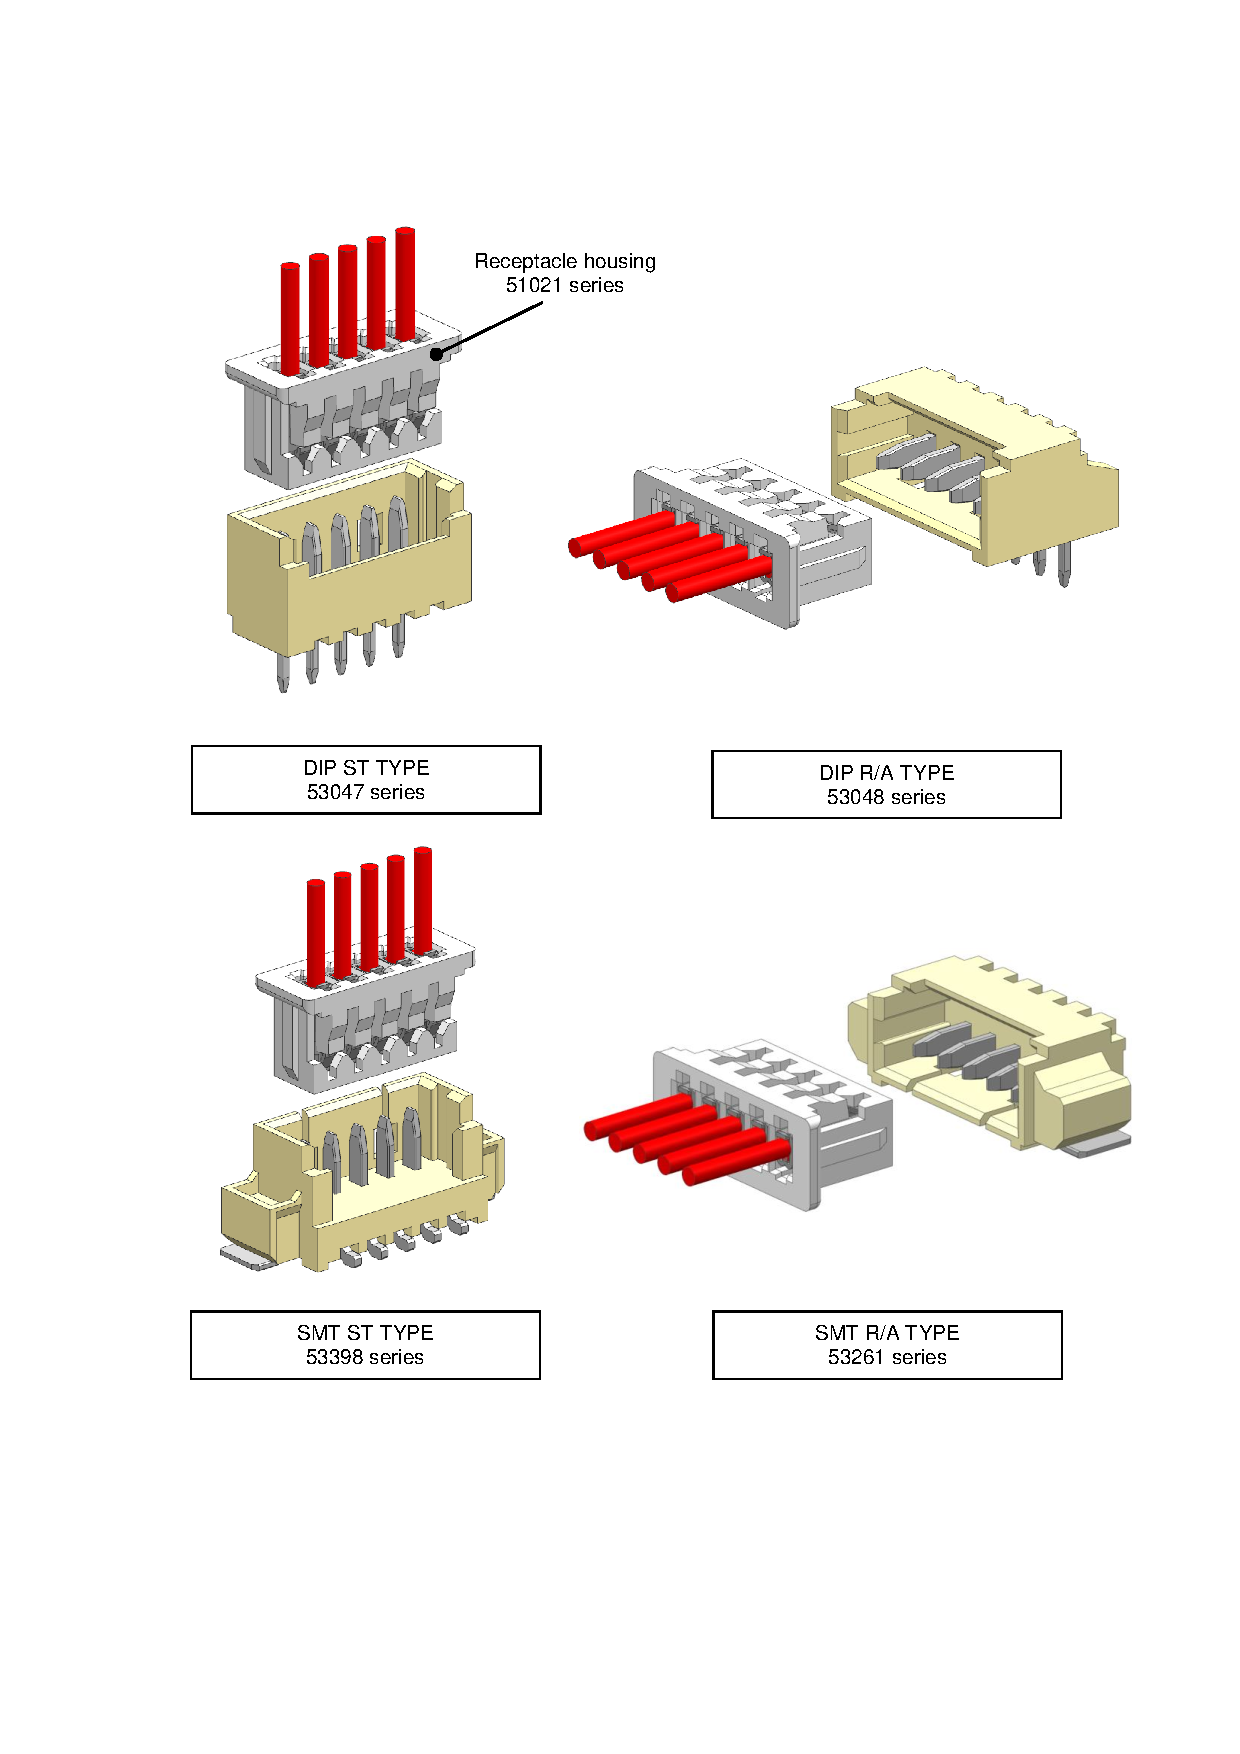
\includegraphics[width=\columnwidth]{51021-APPLICATION-SPECIFICATION.pdf}
    \caption{Molex 51021 连接}
    \label{fig:51021-APPLICATION-SPECIFICATION}
\end{figure}